\begin{figure}
\centering
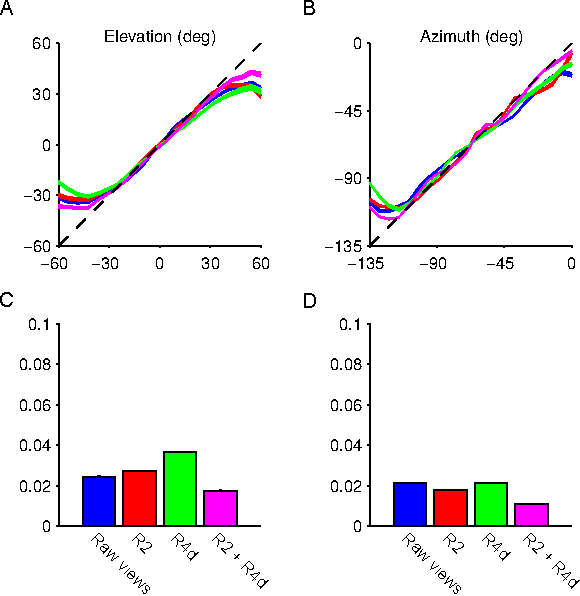
\includegraphics{figures/elaz}
\caption{Analysing the positional information encoded by R2 cells.
Neural networks can be trained to estimate the elevation and azimuth of visual stimuli simultaneously ($N=$~10,000) given the output of the R2 cells.
Networks were trained with raw views ($N=36$~pixels; blue), R2 neurons ($N=28$; red), R4d neurons ($N=14$; green) or R2 and R4 neurons ($N=42$; magenta).
Each of these `types' of network was generated 100 times and average performance was taken.
A and B: Plots of elevation and azimuth of visual stimuli \emph{vs} mean network output for the networks.
The dashed line indicates ideal performance (i.e. $y=x$) and the thickness of the lines at each point shows standard error.
The possible values of elevation and azimuth were constrained by the size of the fruitfly visual field (approx. $120\degree \times 270\degree$).
C and D: Mean square error for each combination of parameter varied and network type.
Standard error is shown, but is very small.
Though performance is best with raw views, it is still good with all the sets of ring neuron inputs.
}
\label{fig:elaz}
\end{figure}
